\documentclass[c,8pt,xcolor...,x11names]{beamer}
\usepackage{icclslides}
\usepackage[latin1]{inputenc}
\usepackage[british]{babel}
\usepackage{amssymb}
\usepackage{latexsym}
\usepackage{rotate}
\usepackage{tikz}
\usepackage{verbatim}
\usepackage{colortbl}
\usepackage{booktabs}
\usepackage{ulem}
% \usepackage{arydshln}
\usepackage{pdfpages}
\usepackage{graphicx} 
\usepackage{tikz}
\usetikzlibrary{positioning}

\tikzstyle{ele} = [circle, text centered, minimum width=1em, minimum height=3ex]

%% Uncomment to activate navigation symbols in the lower right of the pages:
\setbeamertemplate{navigation symbols}{}

\renewcommand{\Myauthor}{Aldo [family name], Tobias John, Patrick Wienh�ft}
\renewcommand{\Mytitle}{The boolean Pythagorean Triples problem}


\author{Aldo [family name]\\ Tobias John\\ Patrick Wienh�ft}

\title{\Mytitle}

\subtitle{subtitle}

%\logo{\includegraphics{logo-tu-ilmenau.jpg}}

\institute{TU Dresden}

\date{date of the presentation}

\usepackage{showexpl} 

\lstloadlanguages{[LaTeX]Tex} 
\lstset{% 
	basicstyle=\ttfamily\small, 
	commentstyle=\itshape\ttfamily\small, 
	showspaces=false, 
	showstringspaces=false, 
	breaklines=true, 
	breakautoindent=true, 
	captionpos=t 
} 

\begin{document} 
	
% alternative title frame
%	\begin{frame}
%	\customtitle
%	\begin{list2}
%		\item What is {\sc Beamer}?
%		\item How to produce a presentation?
%		\item How to create overlays?
%	\end{list2}
%\end{frame}


% title frame
\maketitle


% Aldo's part
\section{Introduction}
\begin{frame}{Example}

	% this is just an idea for an example
	\begin{itemize}
		\item Set of Integers: $ \{1, \ldots, 10\}  $
		\pause
		\item Triples: 
		\begin{flalign*}
		3^2 + 4^2 &= 5^2 &\\ 
		3^2 + 9^2 &= 10^2 &\\
		6^2 + 9^2 &= 10^2
		\end{flalign*}
		\pause
		\item Partition: $ \{1,2,3,4,6,7,8,9 \}, \{5, 10\}  $
	\end{itemize}
	
	
	
\end{frame}

\section{Quick history of the problem}


% Patrik's part
\section{Framework}

\section{Encoding}

\section{Transformations}


% Tobias' part
\section{Cube-and-conquer solving}
\begin{frame}{Cube-and-conquer solving}
	\begin{itemize}
		\item Problem: solving with conflict-driven clause leraning (CDCL) is to slow
		\pause
		\item Solution: use different heuristics $\Rightarrow$ cube-and-conquer solver (C\&C)
	\end{itemize}
	\pause
	\begin{figure}
		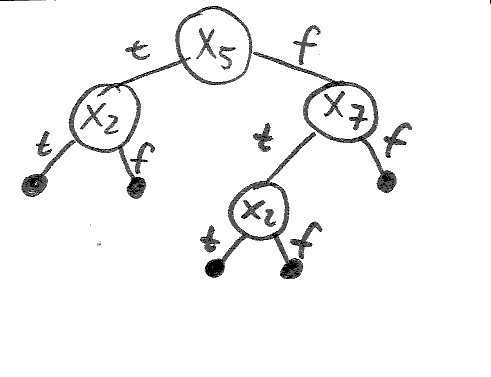
\includegraphics[width=0.5\textwidth]{images/scan1.png} 
		%\caption{Binary branching tree}
	\end{figure}
\end{frame}

\begin{frame}{Runtime}
	\begin{itemize}
		%TODO: add runtime of the algorithm
		\item x time
	\end{itemize}
	\begin{figure}
		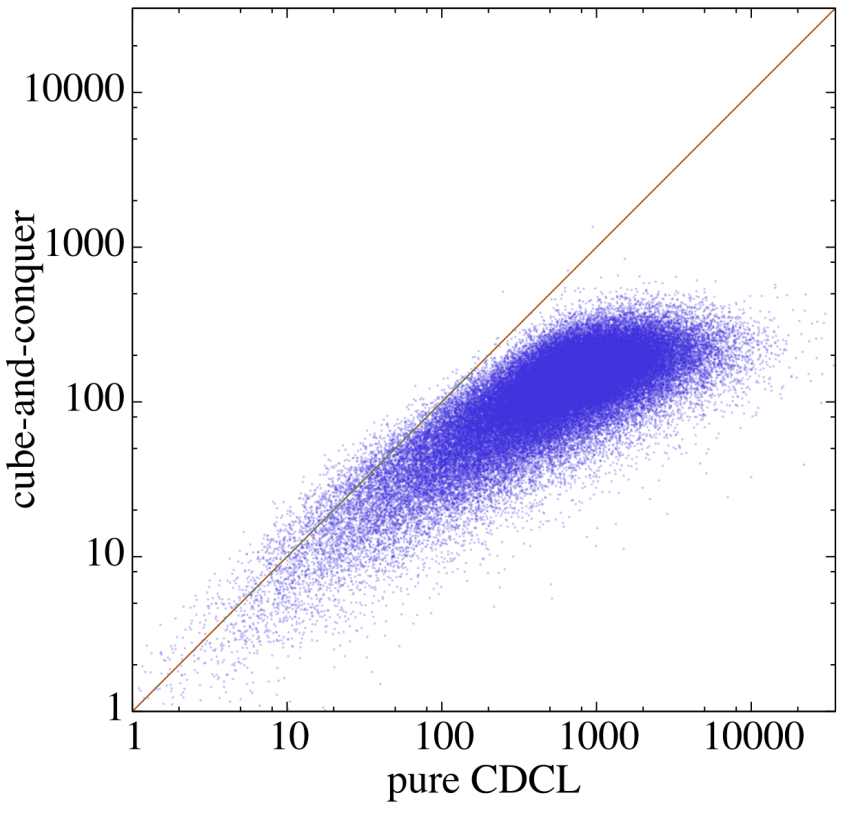
\includegraphics[width=0.5\textwidth]{images/plot1.png} 
		%\caption{runtime of C\&C and CDCL}
	\end{figure}
\end{frame}

\section{Validation}
\begin{frame}{Validation of the program}
	%TODO: add the validation steps
\end{frame}





\end{document}
